% figure for histogram
\begin{figure*}[t]
\centering
\subcaptionbox{\emph{boiler}}
{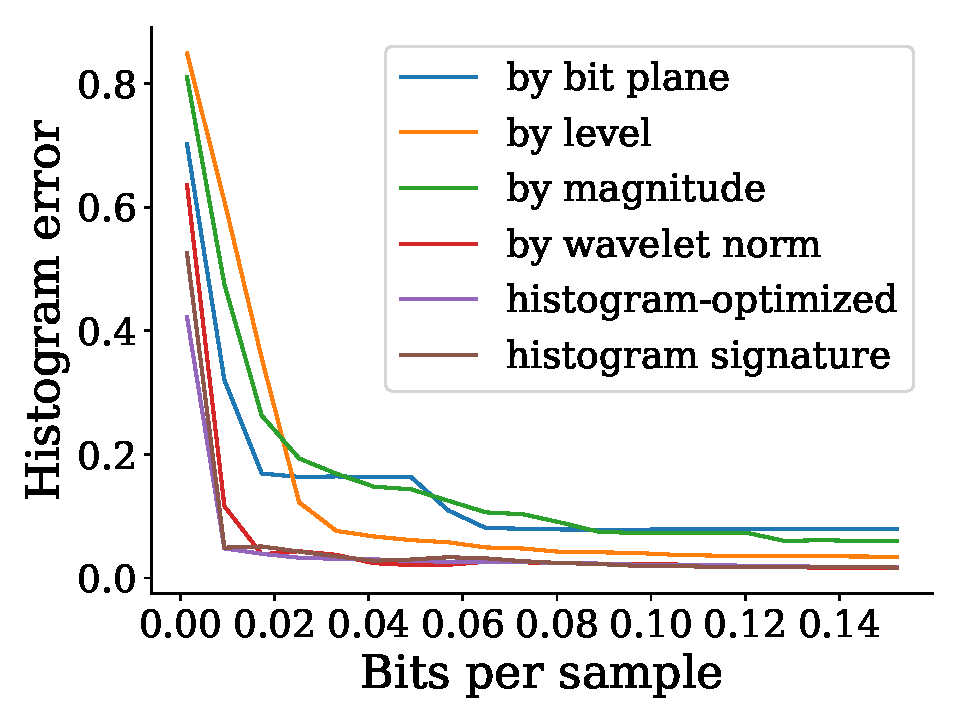
\includegraphics[width=0.24\linewidth]{histogram/histogram-optimized-boiler}\vspace{-0.5em}}
\subcaptionbox{\emph{diffusivity}}
{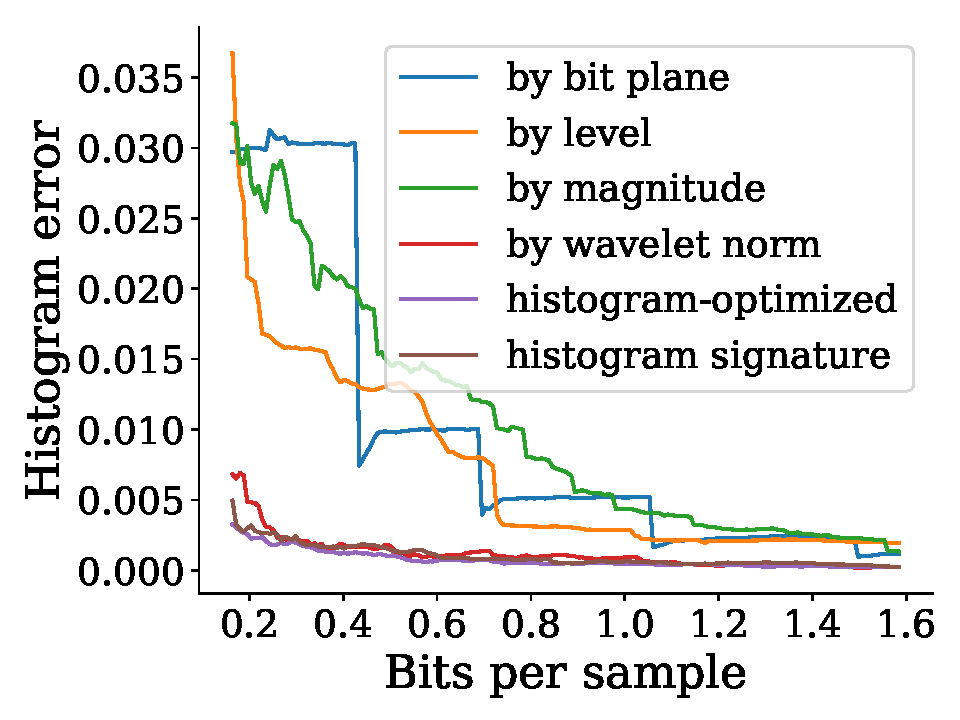
\includegraphics[width=0.24\linewidth]{histogram/histogram-optimized-diffusivity}\vspace{-0.5em}}
\subcaptionbox{\emph{kingsnake}}
{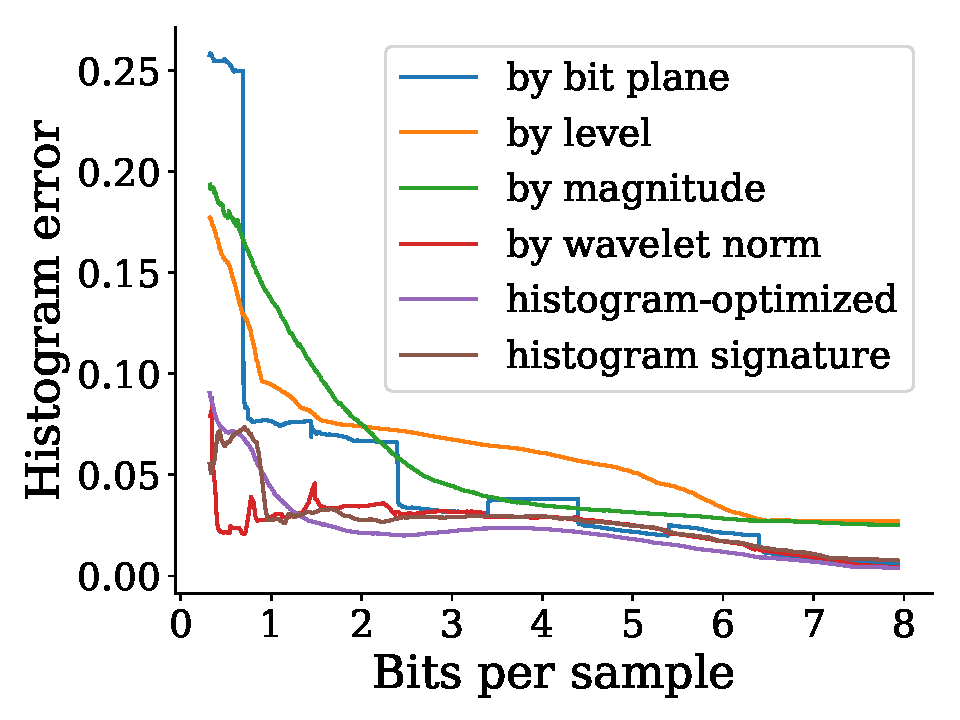
\includegraphics[width=0.24\linewidth]{histogram/histogram-optimized-kingsnake}\vspace{-0.5em}}
\subcaptionbox{\emph{foam}}
{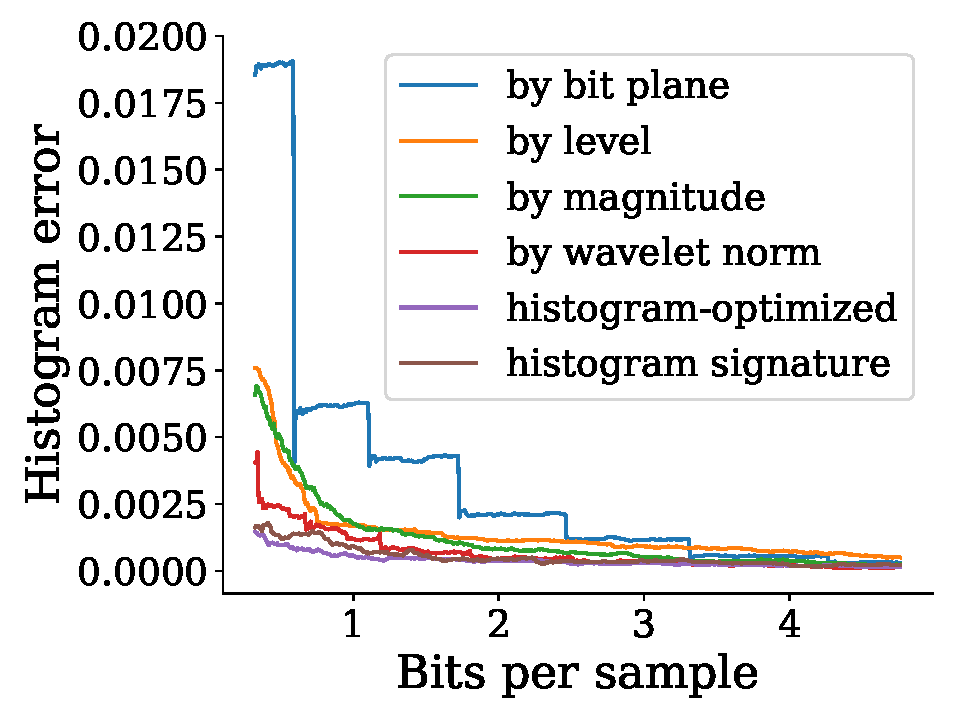
\includegraphics[width=0.24\linewidth]{histogram/histogram-optimized-foam}\vspace{-0.5em}}
\vspace{-0.5em}
\caption{Comparison of histogram errors among streams. Plots are truncated to highlight
differences without hiding important trends. In general, in terms of error, $\shop \approx \shsg
\approx \swav < \slvl, \sbit, \smag$. The erratic behavior at the beginning for \emph{kingsnake}
is likely due to the data being too noisy. The especially poor performances of \sbit for
\emph{boiler} and \emph{foam} are due to the ``shifting'' effect explained in~\Cref{sec:gradient}.
Crossover points between \sbit and \slvl are explained in~\Cref{fig:histogram-explain}.}
\label{fig:histogram-stream-comparison}
\vspace{1em}

\centering
\subcaptionbox{\emph{by level} (\slvl)}{
{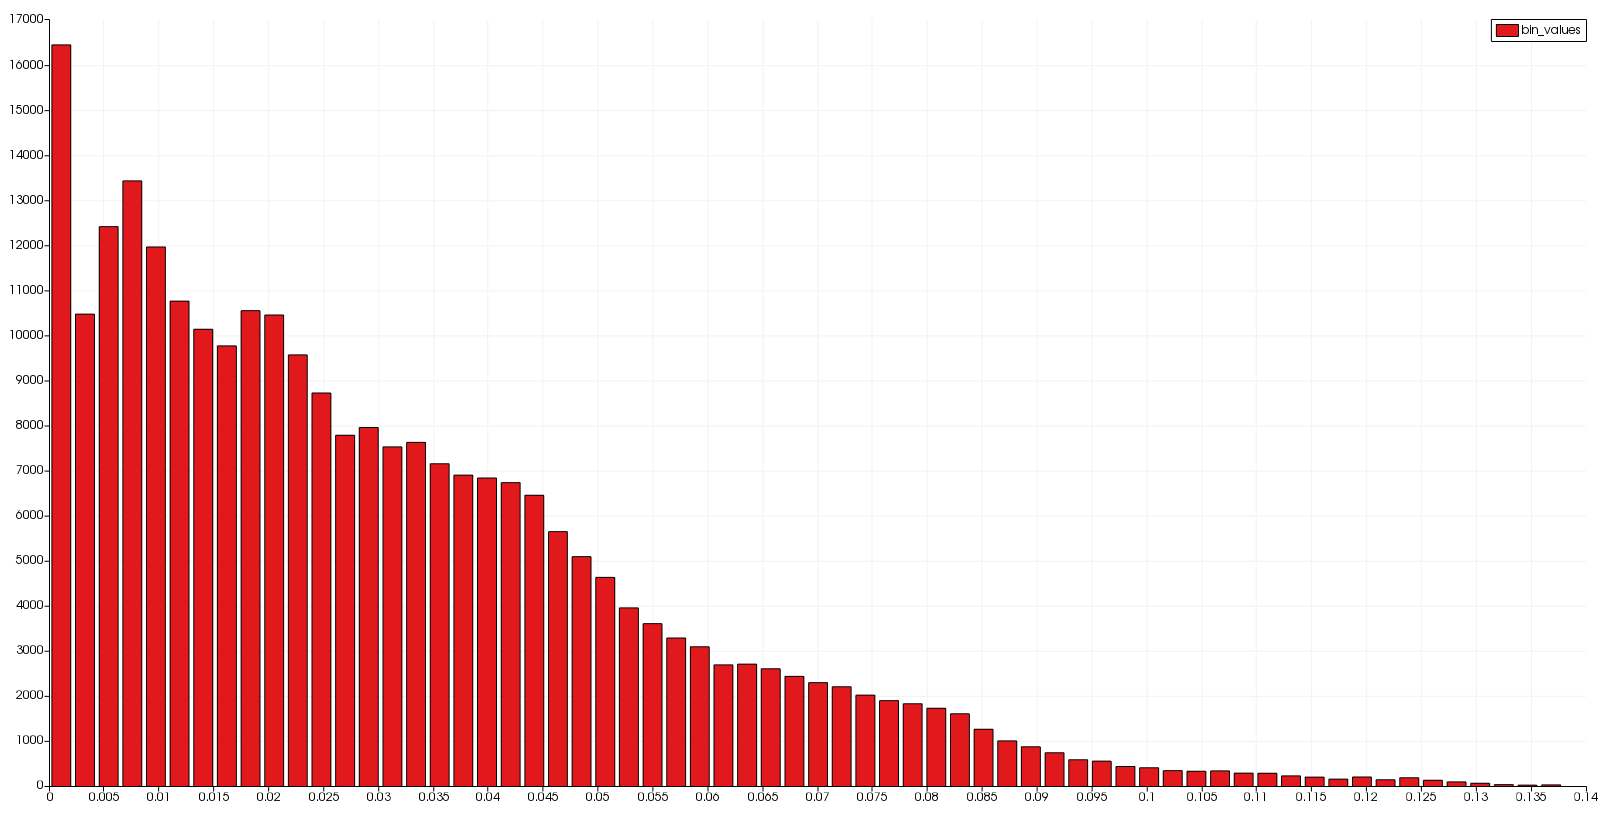
\includegraphics[width=0.158\linewidth]{histogram/histogram-boiler-level}\vspace{-0.5em}}}
\subcaptionbox{\emph{by bit plane} (\sbit)}{
{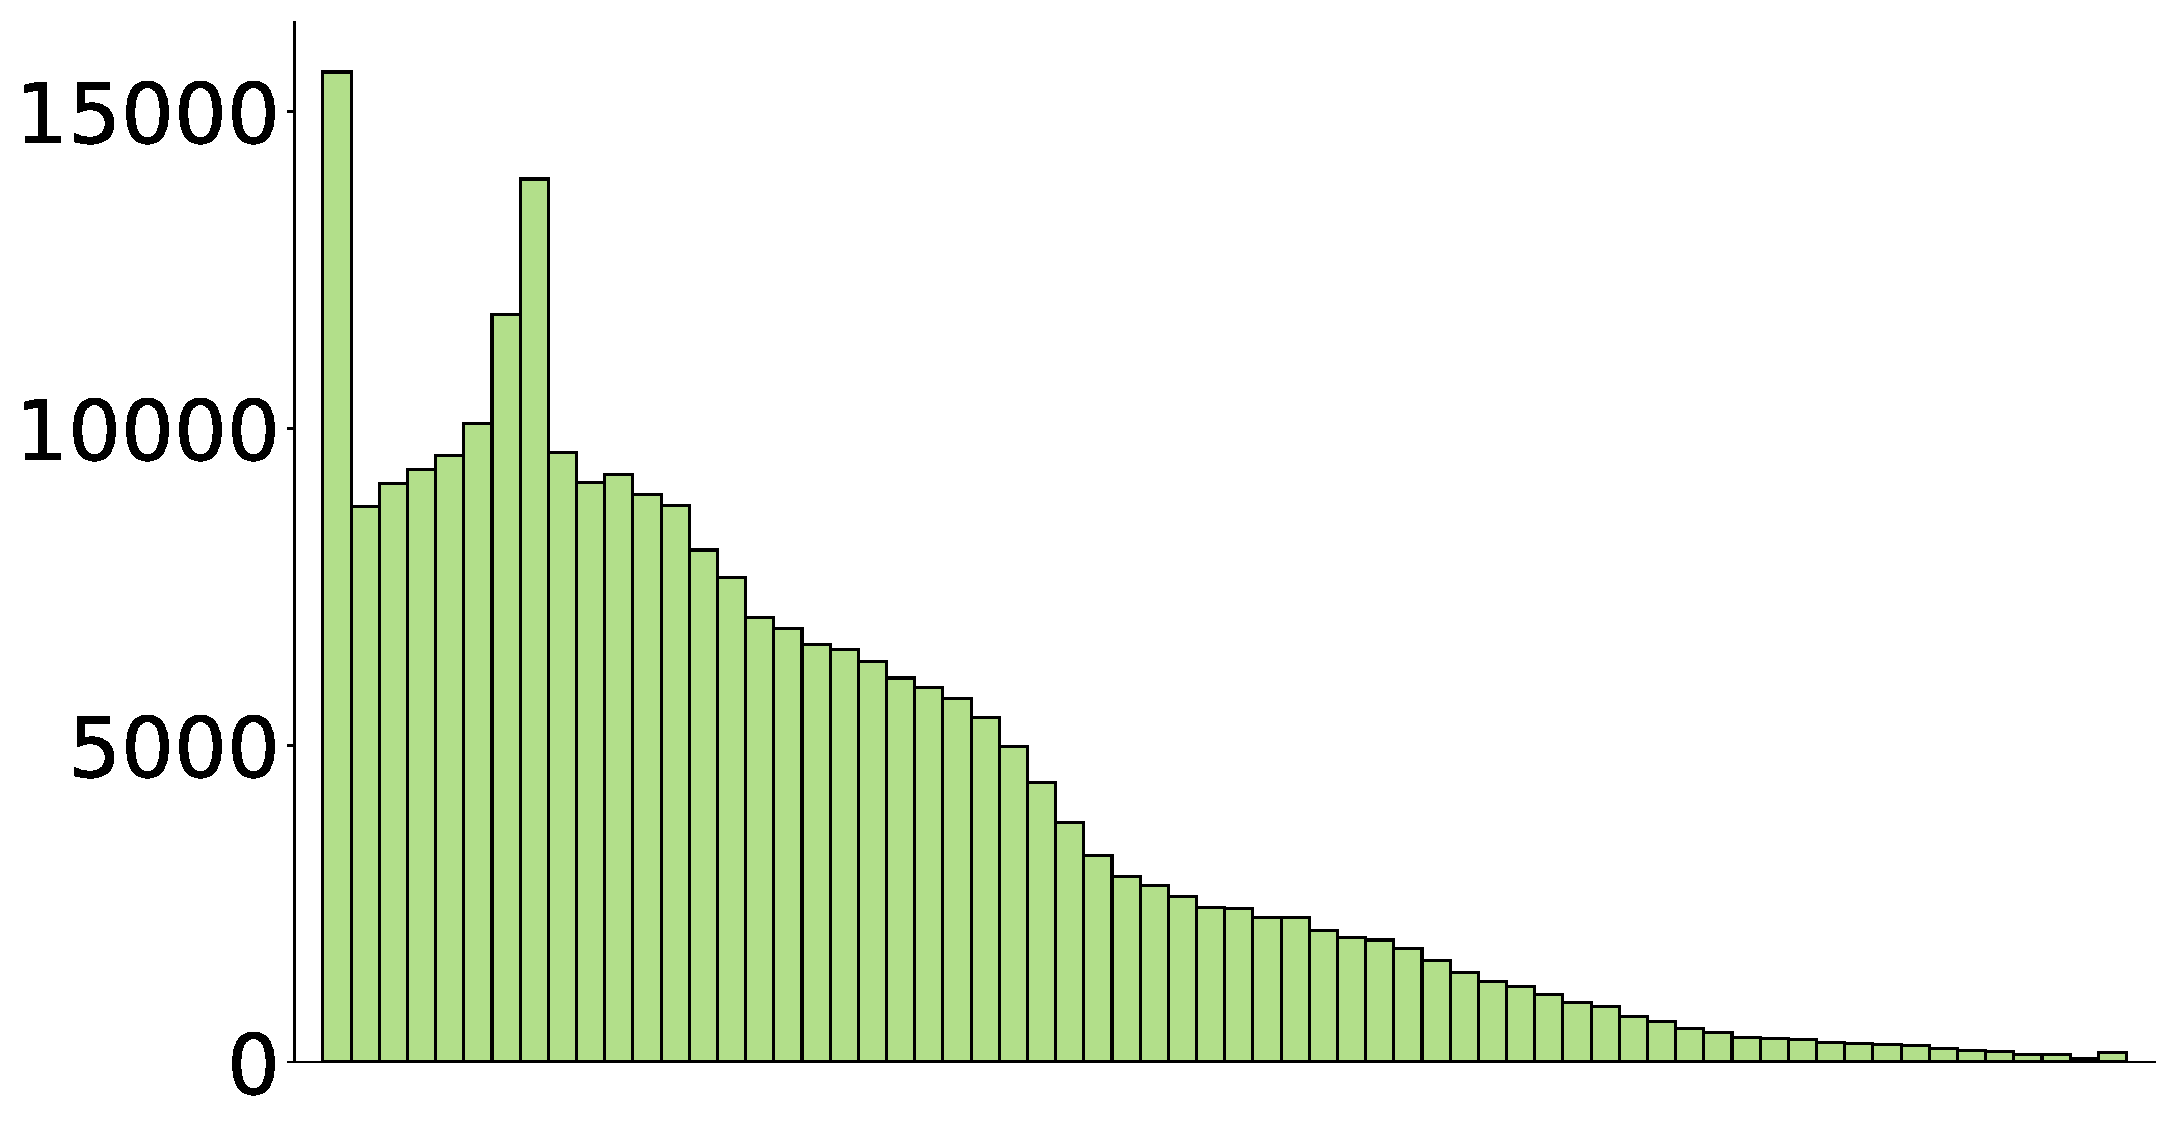
\includegraphics[width=0.158\linewidth]{histogram/histogram-boiler-bit-plane}\vspace{-0.5em}}}
\subcaptionbox{\emph{by magnitude} (\smag)}{
{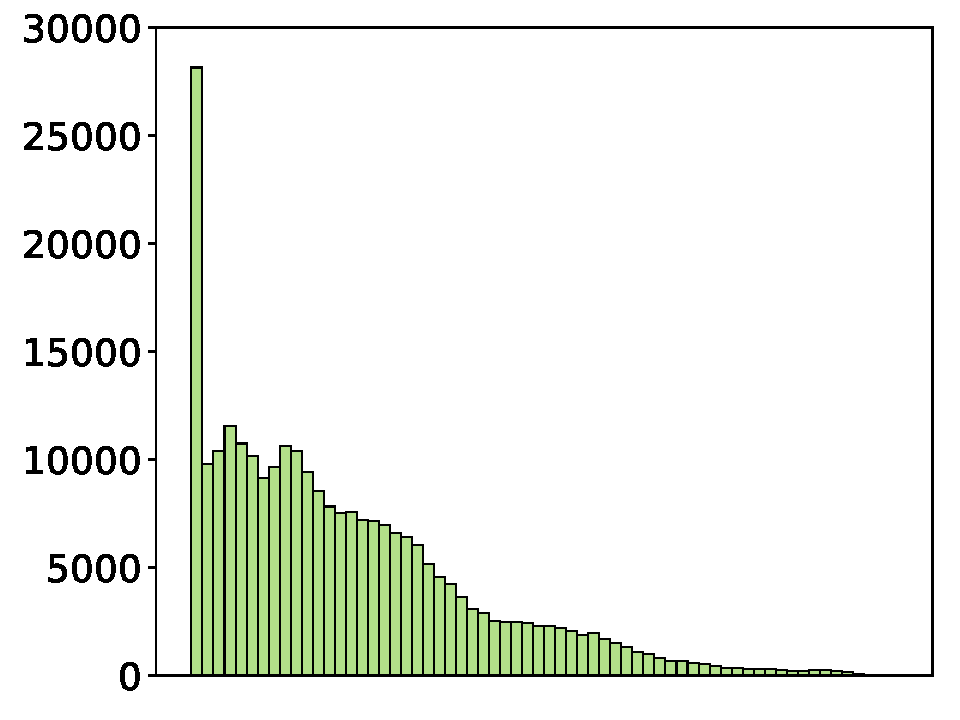
\includegraphics[width=0.158\linewidth]{histogram/histogram-boiler-magnitude}\vspace{-0.5em}}}
\subcaptionbox{\emph{by wavelet norm} (\swav)}{
{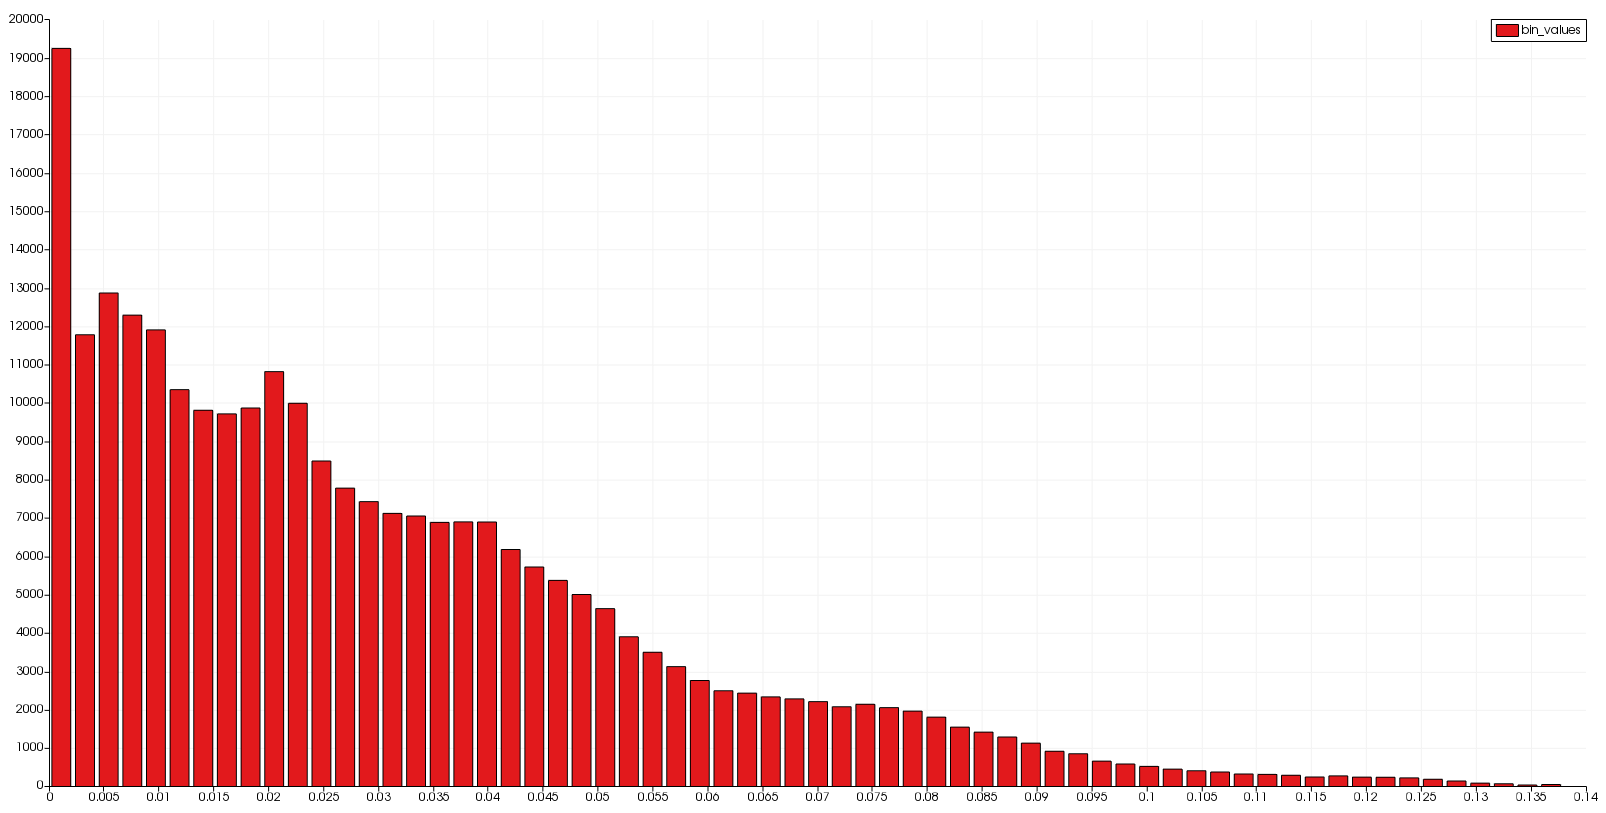
\includegraphics[width=0.158\linewidth]{histogram/histogram-boiler-wavelet-norm}\vspace{-0.5em}}}
\subcaptionbox{\emph{by signature} (\shsg)}{
{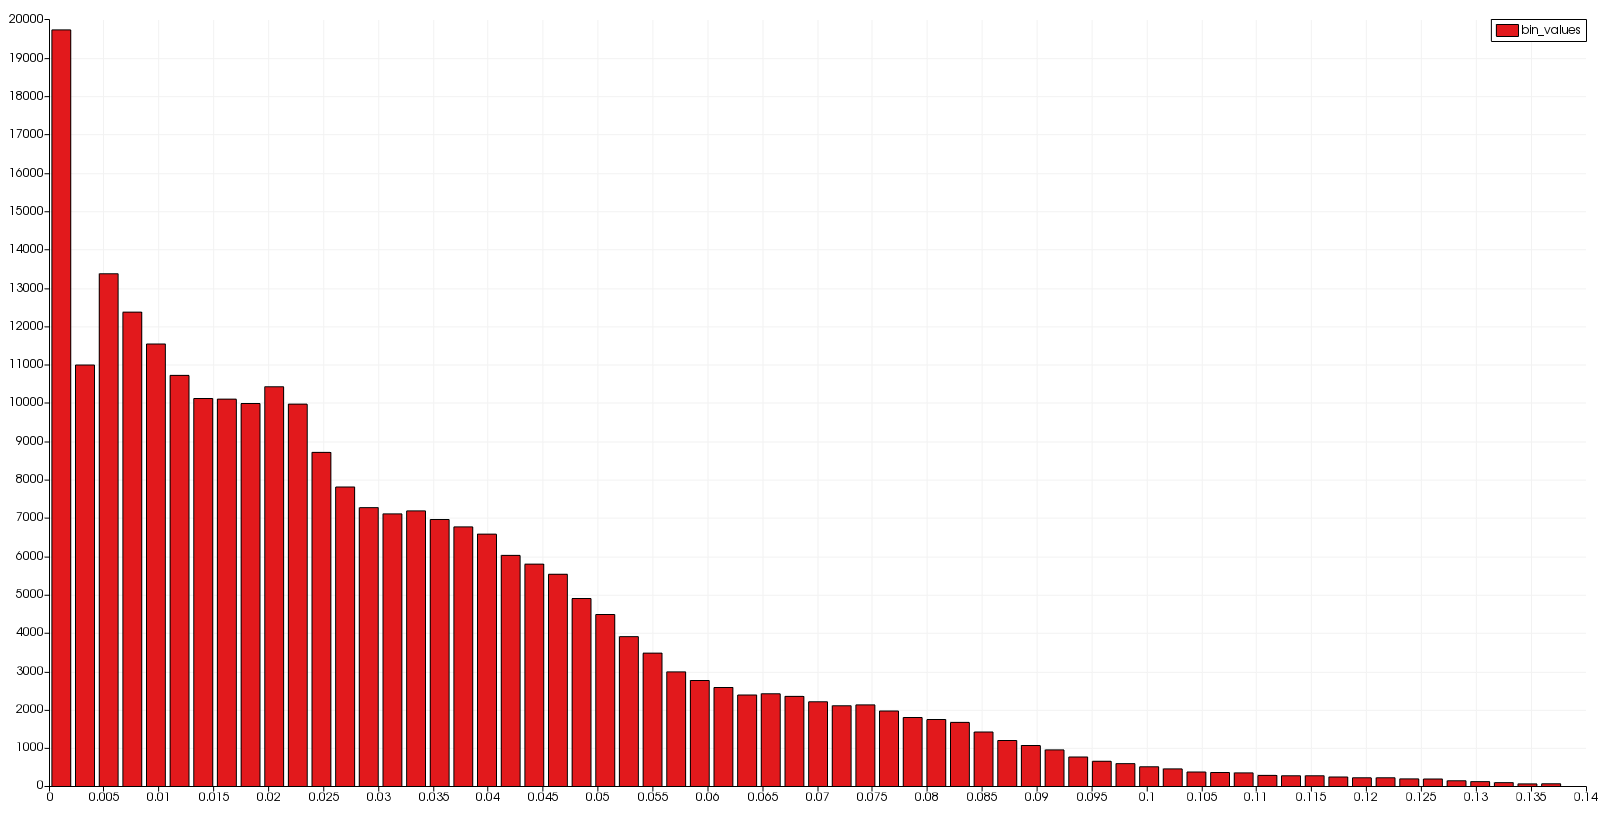
\includegraphics[width=0.158\linewidth]{histogram/histogram-boiler-signature}\vspace{-0.5em}}}
\subcaptionbox{\emph{reference}}{
{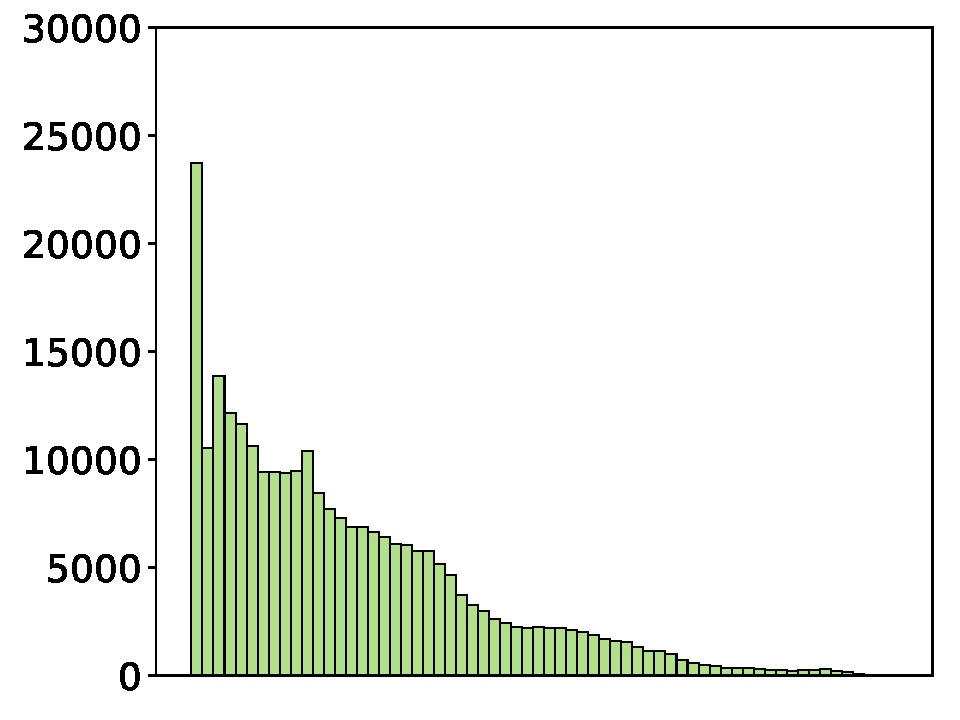
\includegraphics[width=0.158\linewidth]{histogram/histogram-boiler-groundtruth}\vspace{-0.5em}}}
\vspace{-0.5em}
\caption{Histograms of the \emph{boiler} data set, reconstructed at 0.3 bps. \slvl, \swav, and
\shsg produce histograms that share a shape similar to the reference histogram, with most of the
peaks and valleys preserved. In contrast, \sbit produces a spurious peak not found in the
reference. Finally, \smag's histogram has a widely skewed distribution where too many values fall
into the first bin.}
\label{fig:histograms-boiler}
\vspace{-1em}
\end{figure*}

\begin{figure}[!t]
\centering
\subcaptionbox{with leading zero packets}
{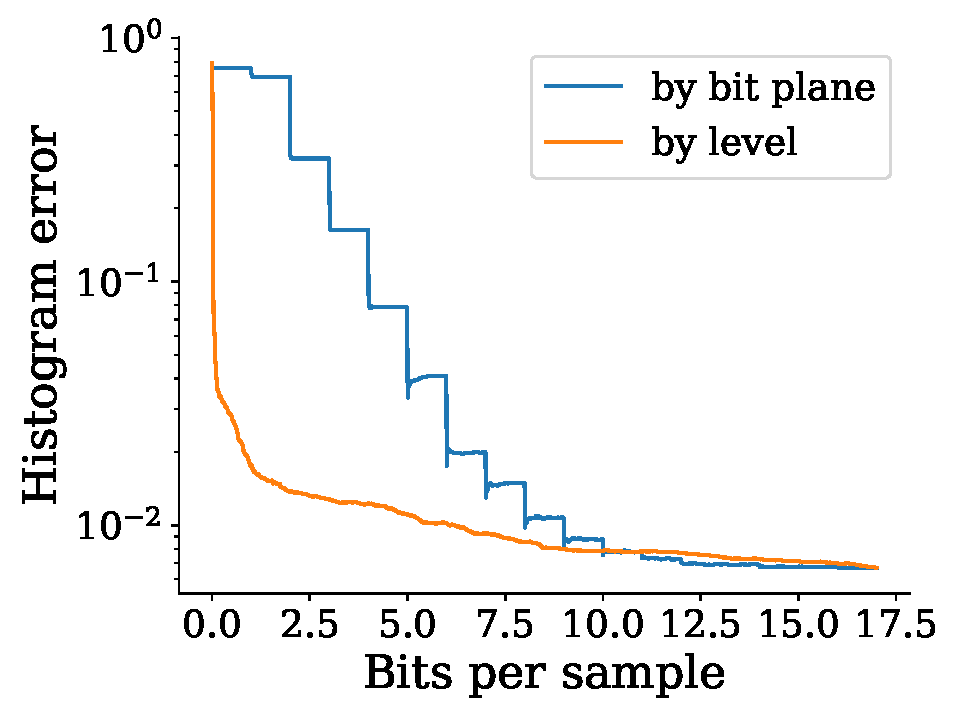
\includegraphics[width=0.48\linewidth]{histogram/histogram-explain-boiler-wlz}\vspace{-0.5em}}
\subcaptionbox{without leading zero packets}
{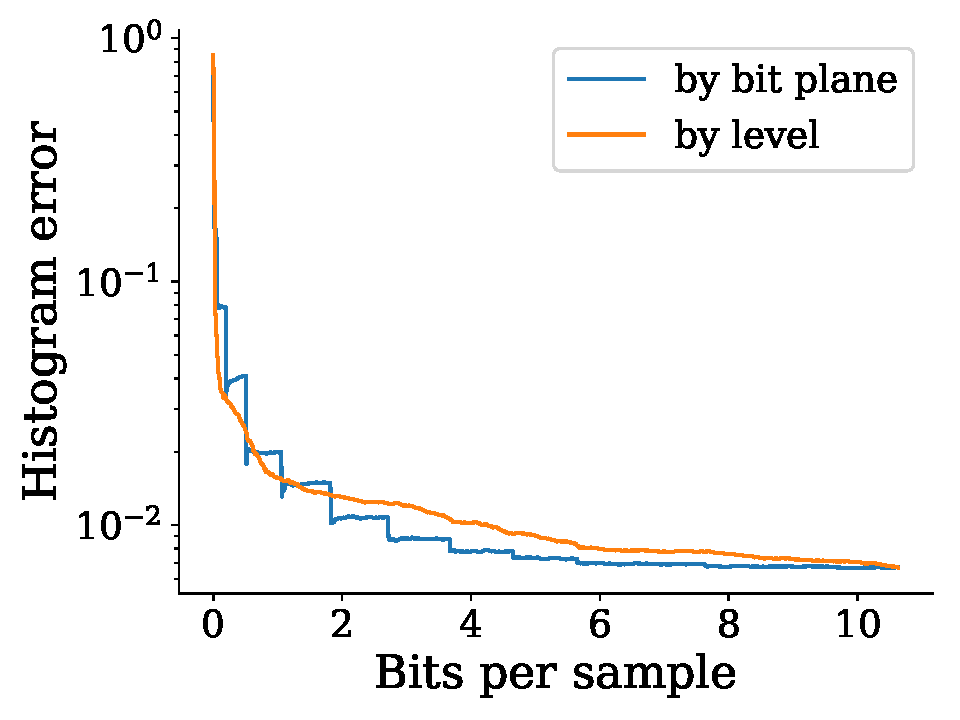
\includegraphics[width=0.48\linewidth]{histogram/histogram-explain-boiler}\vspace{-0.5em}}
\vspace{-0.5em}
\caption{Histogram error curves produced by \sbit and \slvl, for \emph{boiler}, with and without
leading zero bits. The vertical axis is in log scale. The error for \sbit reduces in a stair-step
fashion, where each step corresponds to a new bit plane streamed. \sbit benefits significantly more
from the removal of leading zero bits (the blue curve shifts more to the left).}
\label{fig:histogram-explain}
\vspace{-1.5em}
\end{figure}

% figure for isosurface
\begin{figure*}[t]
\centering
\subcaptionbox{\em pressure, isovalue=0.2}
{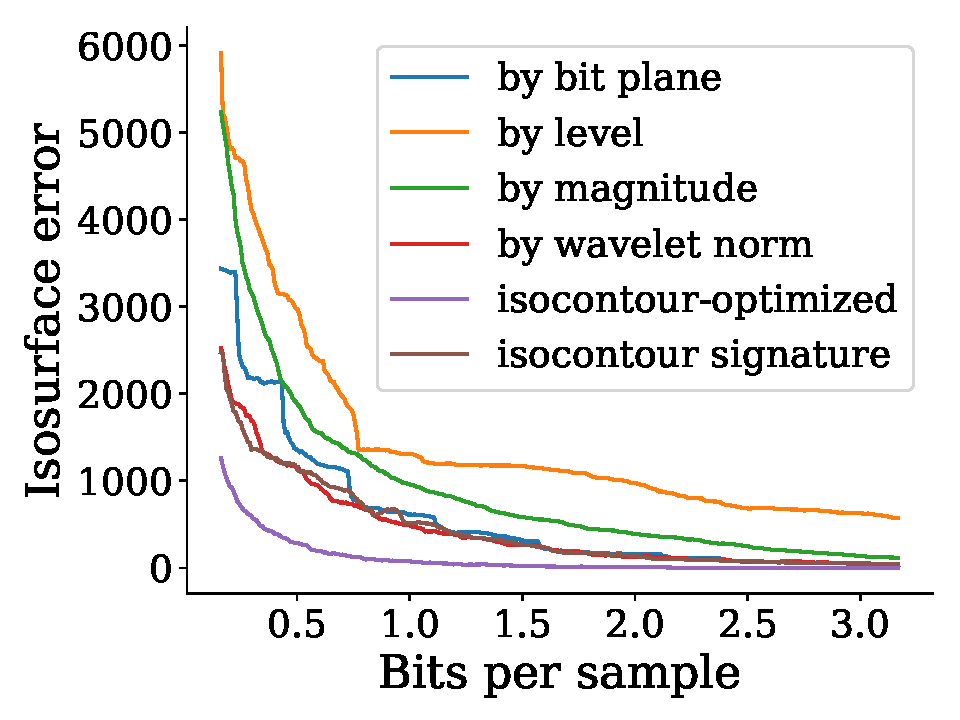
\includegraphics[width=0.24\linewidth]{isocontour/isocontour-optimized-pressure}\vspace{-0.5em}}
\subcaptionbox{\em kingsnake, isovalue=106}
{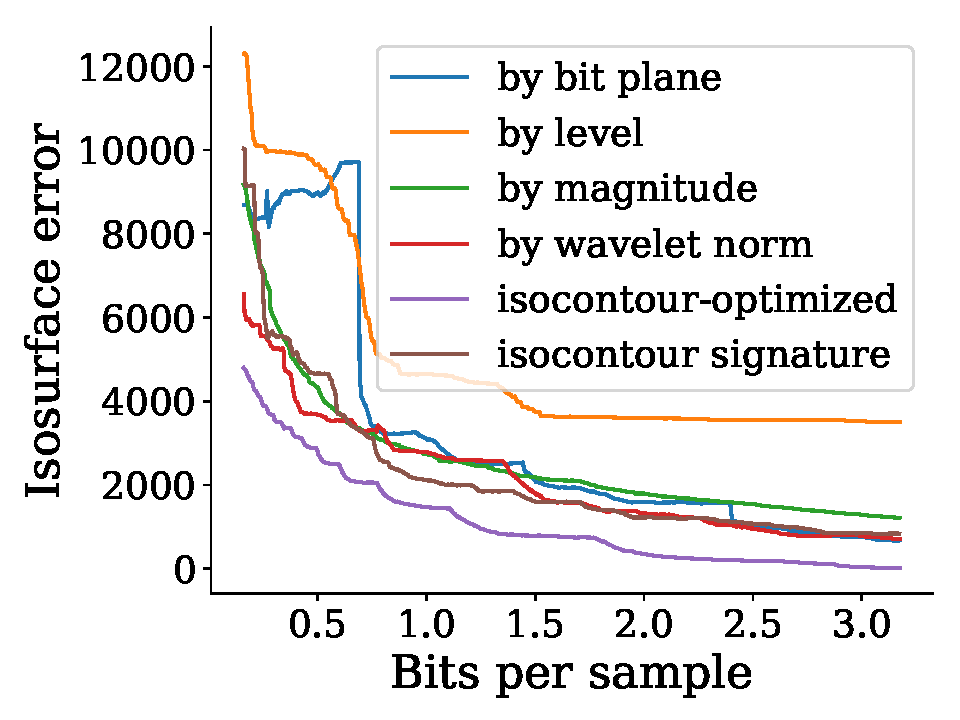
\includegraphics[width=0.24\linewidth]{isocontour/isocontour-optimized-kingsnake}\vspace{-0.5em}}
\subcaptionbox{\em plasma, isovalue=2}
{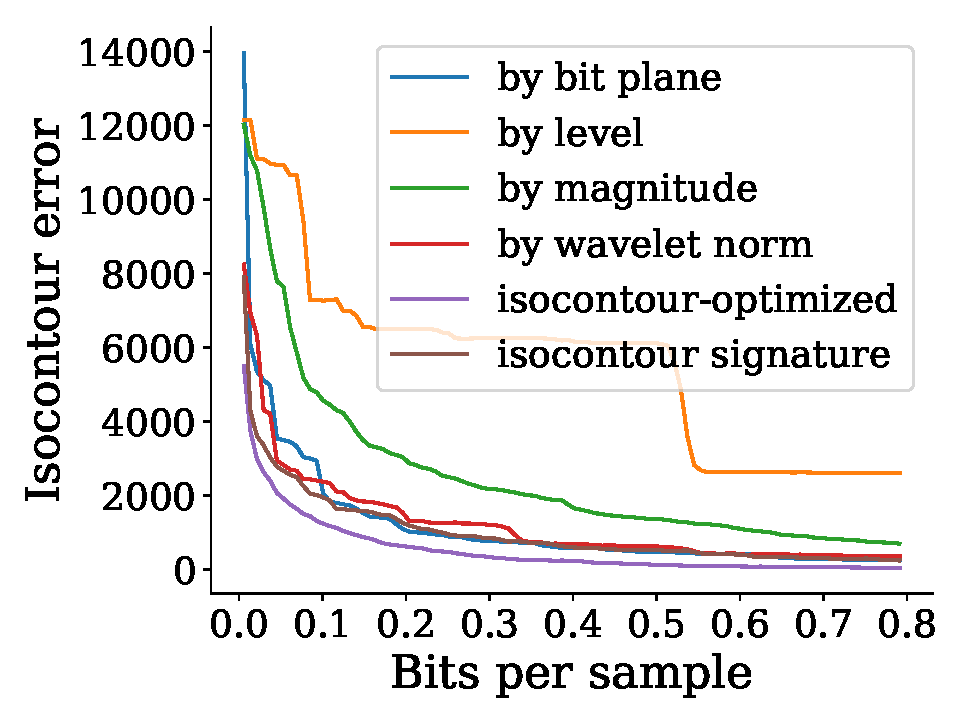
\includegraphics[width=0.24\linewidth]{isocontour/isocontour-optimized-plasma}\vspace{-0.5em}}
\subcaptionbox{\em turbulence, isovalue=2}
{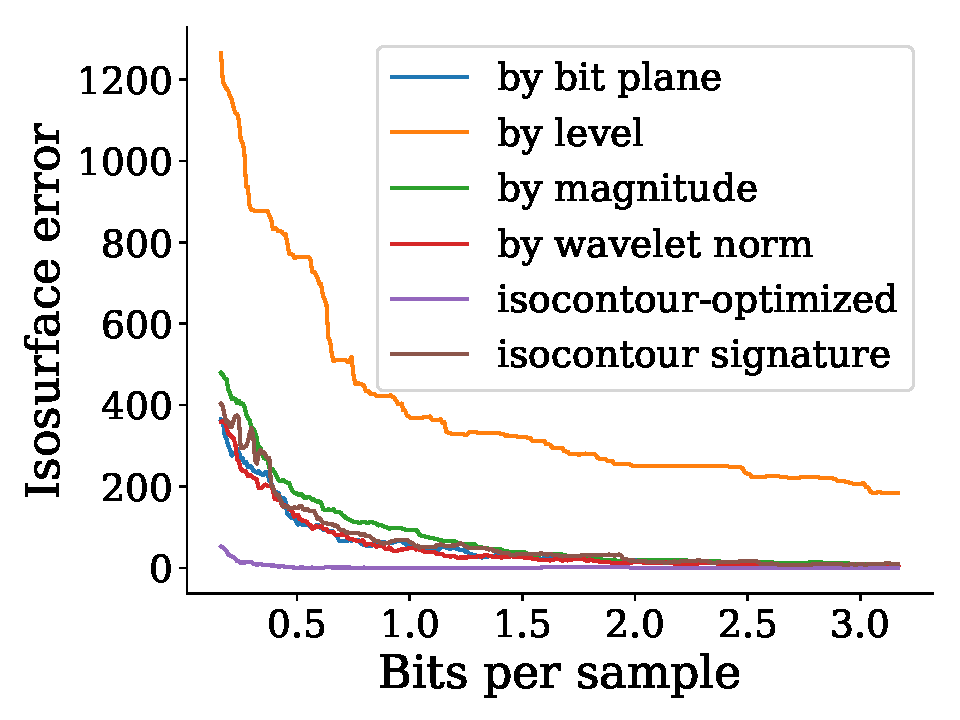
\includegraphics[width=0.24\linewidth]{isocontour/isocontour-optimized-turbulence}\vspace{-0.5em}}
\vspace{-0.5em}
\caption{Comparison of isosurface errors among streams. Plots are truncated to highlight differences
without hiding important trends. The trend in error is $\siop < \sisg \approx \swav < \sbit < \smag
<< \slvl$.}\label{fig:isocontour-plots}
\vspace{1em}

\centering
\subcaptionbox{\emph{by level} ($s_{lvl}$)}
{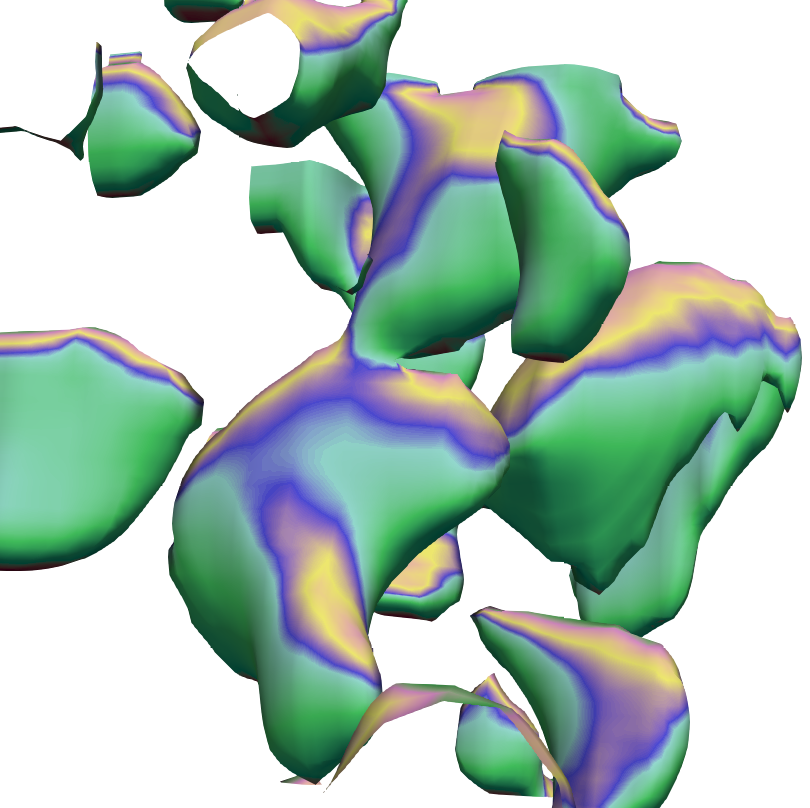
\includegraphics[width=0.16\linewidth]{isocontour/isocontour-level}\vspace{-0.5em}}
\subcaptionbox{\emph{by bit plane} ($s_{bit}$)}
{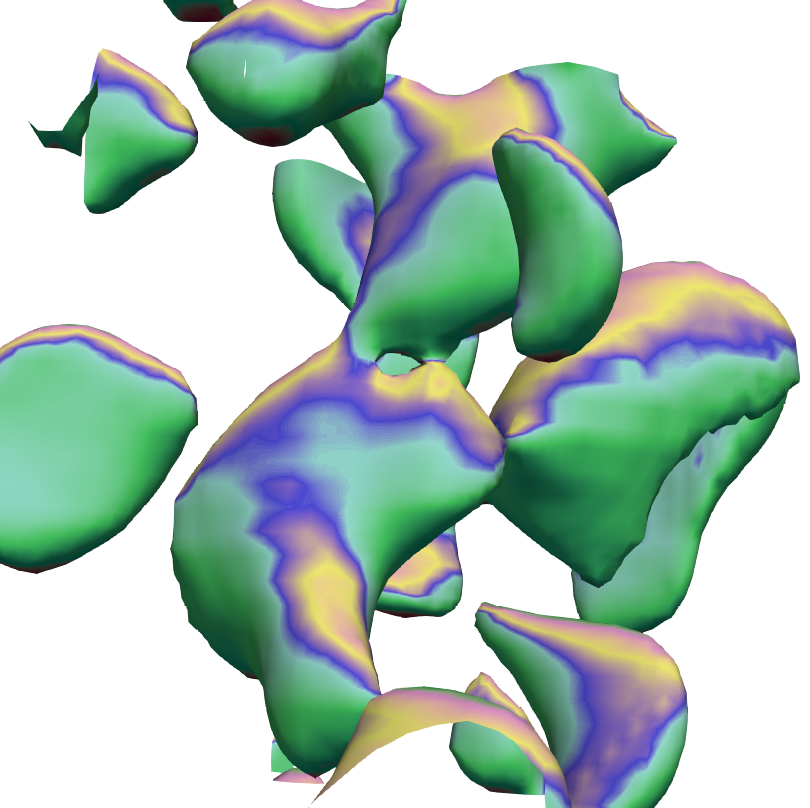
\includegraphics[width=0.16\linewidth]{isocontour/isocontour-bit-plane}\vspace{-0.5em}}
\subcaptionbox{\emph{by wavelet norm} ($s_{wav}$)}
{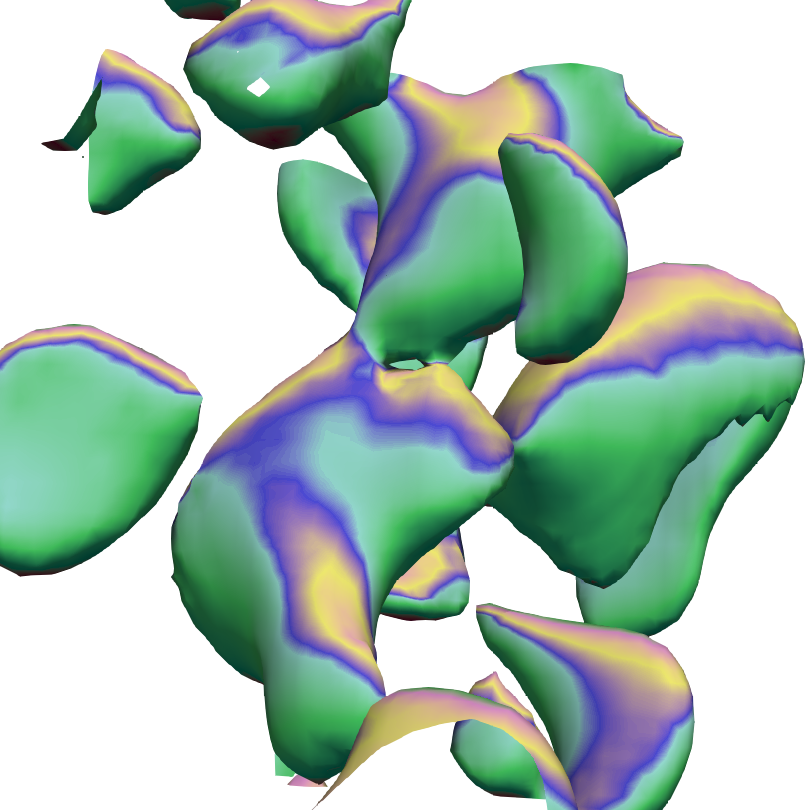
\includegraphics[width=0.16\linewidth]{isocontour/isocontour-wavelet-norm}\vspace{-0.5em}}
\subcaptionbox{\emph{by magnitude} ($s_{mag}$)}
{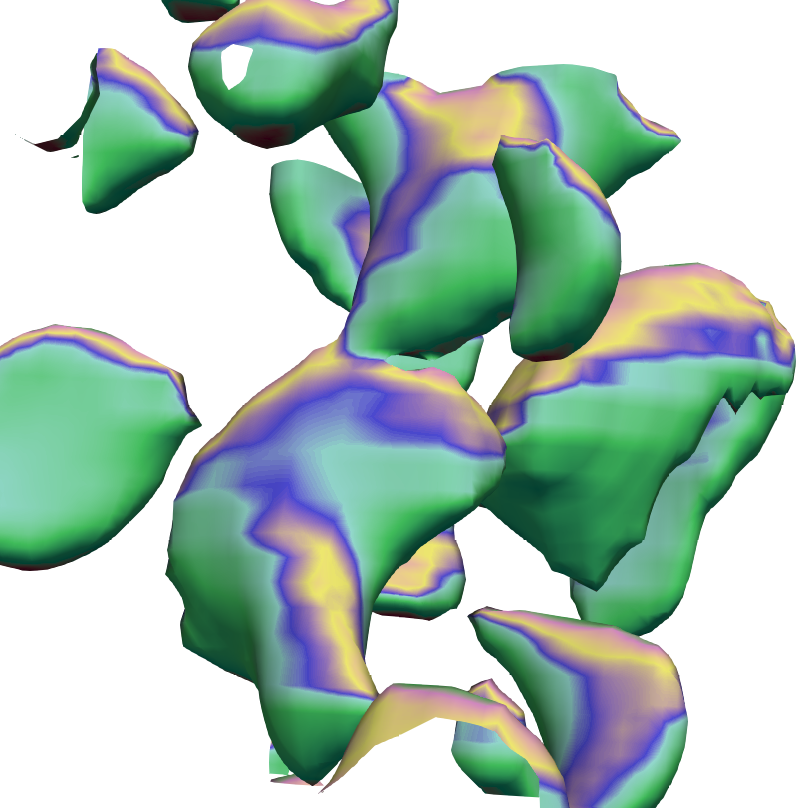
\includegraphics[width=0.16\linewidth]{isocontour/isocontour-magnitude}\vspace{-0.5em}}
\subcaptionbox{\emph{by signature} ($s_{iso-sig}$)}
{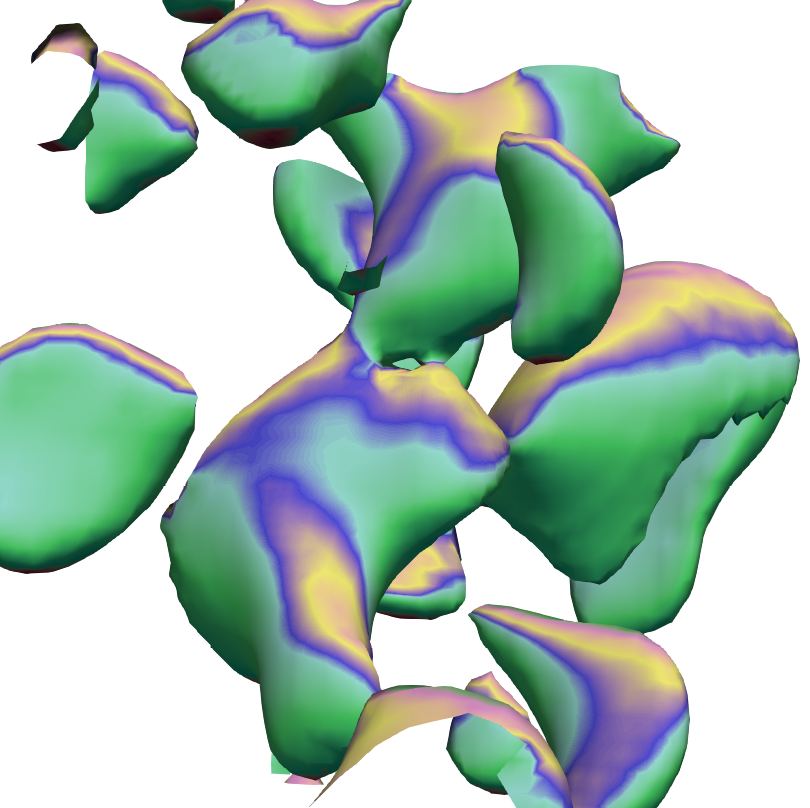
\includegraphics[width=0.16\linewidth]{isocontour/isocontour-signature}\vspace{-0.5em}}
\subcaptionbox{\emph{reference}}
{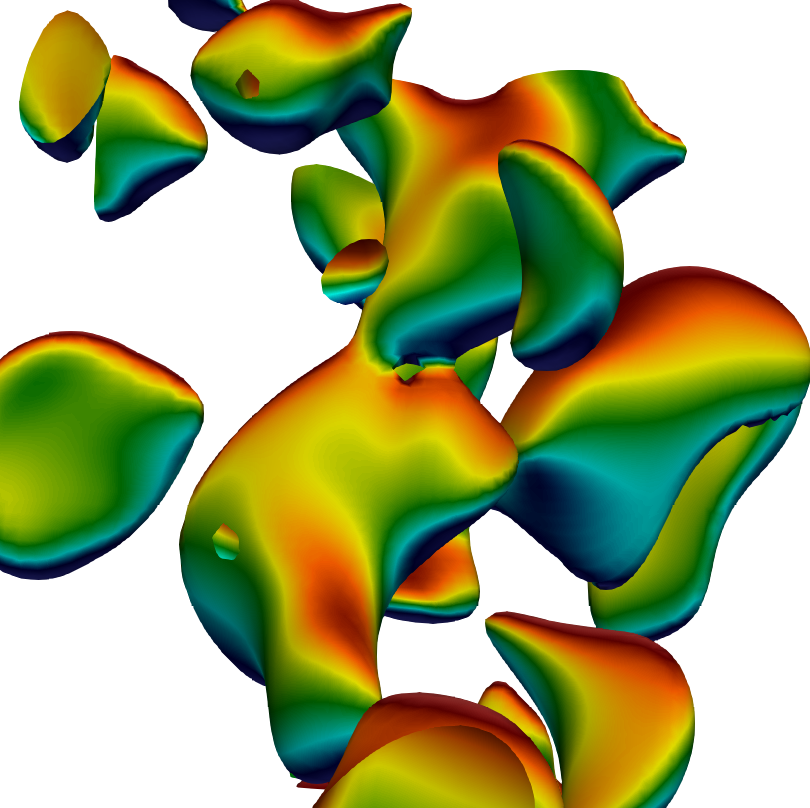
\includegraphics[width=0.16\linewidth]{isocontour/isocontour-groundtruth}\vspace{-0.5em}}
\vspace{-0.5em}
\caption{Rendering of isosurfaces at isovalue of 0.2, at 0.6 bps, for the \emph{pressure} data set.
The surfaces are colored by the $x$-component of the normal vector at each point. \swav and
\sisg produce surfaces that are closest to the reference, followed by \sbit, \smag, and \slvl.}
\label{fig:isocontour-surfaces-pressure}
\vspace{-1.5em}
\end{figure*}


\subsection{Histogram Computation}\label{sec:histogram}

A histogram succinctly summarizes the distribution of sample values, and thus it is useful as a
cursory ``look'' into the data and in guiding further analysis. For example, it can be used to guide
the selection of colors and opacities in a transfer function.

To decide on an error metric to compare histograms, we experimented with several popular metrics
such as Kolmogorov-Smirnov~\cite{smirnov1948}, Kullback-Leibler~\cite{kullback1951}, and Earth
Mover's Distance~\cite{emd1998}, among others~\cite{Hellinger1909,Bhattacharyya1943}. We chose
histogram intersection~\cite{histogram_intersection1991} as the metric of choice, because it is fast
to compute and is reasonably insensitive to changes in precision, as well as the number of bins. The
intersection distance between two histograms $H_1$ and $H_2$ is defined as
$\err(H_1,H_2)=1-\sum_{i}{\min{(H_1(i),H_2(i))}}$ (the sum is over all bins $i$). Every histogram is
normalized by dividing the value in each bin by the total number of samples. We decided that the
error metric should take into account both the histogram shapes and the range of values, and we
clamped the range of values in reconstructed functions to that of the original function, so that
corresponding histogram bins, i.e., $H_1(i)$ and $H_2(i)$, share the same range.

As before, for each data set, we use~\Cref{alg:greedy} to compute an \shop stream, optimized for
histogram error, and then construct an \shsg from its signature. We plot the error curves for all
relevant streams using the Intersection error metric~(compare
\Cref{fig:histogram-stream-comparison}). We use 64 for the number of bins but note that there exist
no meaningful differences across a wide range of number of bins (from 64 to 512) in our experiments.
In all cases, the group consisting of \sbit, \slvl, and \smag underperforms the other group by a
large margin.

\smag performs poorly, because it ignores regions of smooth variations, which nevertheless count
toward the distribution. \slvl generally outperforms \sbit at low bit rates, although there are
several crossover points between the two curves. As can be seen in~\Cref{fig:histogram-explain},
\slvl outperforms \sbit when leading zero packets are present, because increasing resolution does
not help as much as increasing precision. This is because the histogram is oblivious to spatial
locations of samples (which require resolution to resolve) but is sensitive to sample values (which
require precision). However, when leading zero packets are removed, \sbit benefits significantly
more than \slvl does (for the same reason explained in~\Cref{sec:rmse-optimized}), resulting in the
observed crossovers.

In the latter group, the performances of \swav and \shsg (and even \shop) differ by a negligible
amount. This observation is confirmed in~\Cref{fig:histograms-boiler}, where we plot various
histograms, reconstructed at 0.3 bps, for the \emph{boiler} data set. The histograms produced by
\swav and \shsg have approximately the same shape and are the closest to the reference histogram.
The next best histogram is produced by \slvl, followed by the one produced by \sbit, and finally
\smag. These results suggest that histogram computation benefits from a bit ordering that combines
both resolution and precision, with a strong bias toward precision.
